\documentclass[11pt,a4paper]{article}
\usepackage[margin=1in]{geometry}
\usepackage[T1]{fontenc}
\usepackage[utf8]{inputenc}
\usepackage{lmodern}
\usepackage{hyperref}
\usepackage{enumitem}
\usepackage{xurl}
\usepackage{tikz}
\usepackage{float}
\usetikzlibrary{arrows.meta, positioning, shapes.geometric}
\hypersetup{colorlinks=true,linkcolor=blue,urlcolor=blue}
\newcommand{\codepath}[1]{\path{#1}}
\tikzset{
  box/.style={rectangle,draw,rounded corners,align=center,inner sep=3pt,minimum width=44mm},
  decision/.style={diamond,draw,aspect=2.2,align=center,inner sep=2pt},
  line/.style={-Latex}
}

\title{Phase-2 Deliverable: Adapter Contract}
\author{SIT Engine Documentation}
\date{\today}

\begin{document}
\maketitle

\section{Technical Description}
This deliverable formalizes adapter boundaries so simulator-specific normalization does not leak SIT policy decisions into adapters.

\section{Implementation Fulfillment}
Contract rules are documented in \codepath{Phase-2/ADAPTERS.md}; enforced by \codepath{Phase-2/ingest/ingest_api.py}; consumed by \codepath{Phase-2/sit_engine_phase1.py}.

\section{Design \& Architecture}
\subsection*{Function Attributes}
\begin{itemize}[leftmargin=*]
  \item \texttt{validate\_state\_df()}: Inputs=state intervals with required columns; Outputs=validated state intervals; Side effects=enforces schema + state domain; Failure modes=invalid state label, non-positive duration.
  \item \texttt{validate\_resid\_df()}: Inputs=residency intervals; Outputs=validated residency intervals; Side effects=filters resident rows and validates spans; Failure modes=missing column, bad bounds.
  \item \texttt{BaselineAdapter.load\_state\_intervals()}: Inputs=state CSV path; Outputs=state DataFrame; Side effects=standard ingest adapter bridge; Failure modes=file missing, parse failure.
  \item \texttt{sit\_engine\_phase1.main()}: Inputs=validated interval data + knobs; Outputs=window/summary artifacts; Side effects=sole owner of SIT policy and windowing; Failure modes=policy/config mismatch.
\end{itemize}
\subsection*{Function Execution Details}
\begin{enumerate}[leftmargin=*]
  \item \texttt{validate\_state\_df()}
  \begin{itemize}[leftmargin=*]
    \item Input attributes: state intervals with required columns.
    \item Processing flow: enforces schema + state domain.
    \item Output attributes: validated state intervals.
    \item Failure behavior: invalid state label, non-positive duration.
  \end{itemize}
  \item \texttt{validate\_resid\_df()}
  \begin{itemize}[leftmargin=*]
    \item Input attributes: residency intervals.
    \item Processing flow: filters resident rows and validates spans.
    \item Output attributes: validated residency intervals.
    \item Failure behavior: missing column, bad bounds.
  \end{itemize}
  \item \texttt{BaselineAdapter.load\_state\_intervals()}
  \begin{itemize}[leftmargin=*]
    \item Input attributes: state CSV path.
    \item Processing flow: standard ingest adapter bridge.
    \item Output attributes: state DataFrame.
    \item Failure behavior: file missing, parse failure.
  \end{itemize}
  \item \texttt{sit\_engine\_phase1.main()}
  \begin{itemize}[leftmargin=*]
    \item Input attributes: validated interval data + knobs.
    \item Processing flow: sole owner of SIT policy and windowing.
    \item Output attributes: window/summary artifacts.
    \item Failure behavior: policy/config mismatch.
  \end{itemize}
\end{enumerate}


\subsection*{Diagram A: End-to-End Design Flow}
\begin{figure}[H]
\centering
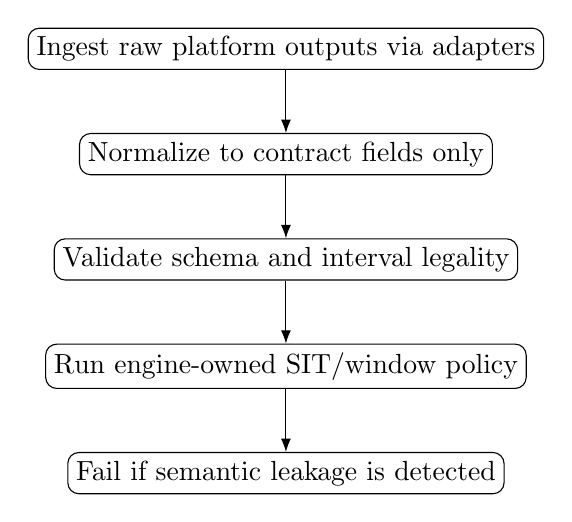
\begin{tikzpicture}[node distance=8mm and 12mm]
\node[box] (a) {Ingest raw platform outputs via adapters};
\node[box, below=of a] (b) {Normalize to contract fields only};
\node[box, below=of b] (c) {Validate schema and interval legality};
\node[box, below=of c] (d) {Run engine-owned SIT/window policy};
\node[box, below=of d] (e) {Fail if semantic leakage is detected};
\draw[line] (a) -- (b);
\draw[line] (b) -- (c);
\draw[line] (c) -- (d);
\draw[line] (d) -- (e);
\end{tikzpicture}
\caption{Deliverable 03: End-to-End Design Flow}
\end{figure}

\subsection*{Diagram B: Function Interaction and Attribute Flow}
\begin{figure}[H]
\centering
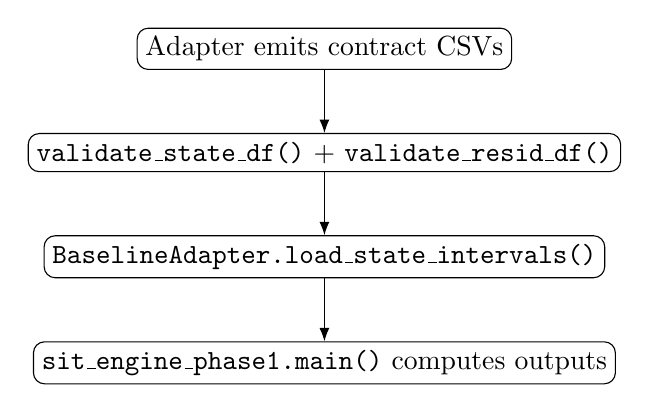
\begin{tikzpicture}[node distance=8mm and 12mm]
\node[box] (fa) {Adapter emits contract CSVs};
\node[box, below=of fa] (fb) {\texttt{validate\_state\_df()} + \texttt{validate\_resid\_df()}};
\node[box, below=of fb] (fc) {\texttt{BaselineAdapter.load\_state\_intervals()}};
\node[box, below=of fc] (fd) {\texttt{sit\_engine\_phase1.main()} computes outputs};
\draw[line] (fa) -- (fb);
\draw[line] (fb) -- (fc);
\draw[line] (fc) -- (fd);
\end{tikzpicture}
\caption{Deliverable 03: Function Interaction and Attribute Flow}
\end{figure}

\end{document}
